\section{Architettura}
\label{architettura}

\subsection{Struttura del database}

Vi sono due tipologie di database:
\begin{itemize}
	\item Database sul server cloud di vision: contiene i dati di autenticazione degli utenti di moviORDER e i dati necessari ad accedere ai database aziendali;
	\item Database aziendali: sono i database contenuti nei server delle varie aziende o nel server cloud di vision nel caso in cui le aziende non abbiano a disposizione un server. Contengono informazioni sugli articoli venduti, sui codici a barre degli articoli, sulle testate di documento e sulle righe di documento. Inoltre contengono le informazioni anagrafiche sui clienti dell'azienda.
\end{itemize}

Il database sul server cloud di vision è chiamato \textbf{mvo_CommonDB} e contiene due tabelle:
\begin{itemize}
	\item \textbf{Users}: contiene le credenziali di autenticazione degli utenti di moviORDER. I campi sono i seguenti:
		\begin{itemize}
			\item \textbf{UserName (PK)}: è lo username dell'utente;
			\item \textbf{Password}: è la password associata allo username;
			\item \textbf{CodAzienda}: è il codice dell'azienda fornitrice dell'utente;
			\item \textbf{EmailU}: è l'indirizzo e-mail dell'utente;
			\item \textbf{Bloccato}: è un flag booleano che indica se l'utente è stato bloccato. Se un utente è stato bloccato, non gli sarà possibile accedere a moviORDER.
		\end{itemize}
	\item \textbf{Aziende}: contiene i dati delle aziende fornitrici i quali clienti utilizzano moviORDER. I campi sono i seguenti:
		\begin{itemize}
			\item \textbf{CodAzienda (PK)}: è il codice univoco dell'azienda;
			\item \textbf{Path}: è la stringa di connessione al database aziendale contenuto sul server cloud di vision o su un server dell'azienda. La stringa deve avere la seguente struttura: \textit{vision.cloudapp.net:1500;databaseName=mvo_aziendaASS;user=ass;password=ass}, dove:
				\begin{itemize}
					\item \textit{vision.cloudapp.net:8080} è l'indirizzo del server dove è contenuto il database;
					\item \textit{databaseName} è il nome del database al quale ci si vuole collegare;
					\item \textit{user} è il nome utente per accedere al database;
					\item \textit{password} è la password associata a \textit{user}.
				\end{itemize}
			\item \textbf{EmailA}: è l'indirizzo e-mail dell'azienda;
			\item \textbf{Host}: è l'indirizzo del server SMTP;
			\item \textbf{Port}: è la posta del server SMTP;
			\item \textbf{Username}: è lo username per accedere al server SMTP;
			\item \textbf{Password}: è la password per accedere al sercer SMTP.
		\end{itemize}
\end{itemize}

Il database aziendale ha la stessa struttura per ogni azienda e può risiedere sul server cloud di vision oppure su un server dell'azienda fornitrice. Il database aziendale contiene le seguenti tabelle:
\begin{itemize}
	\item \textbf{Art}: contiene i dati degli articoli venduti dall'azienda. I campi sono i seguenti:
		\begin{itemize}
			\item \textbf{Id_Art}: codice per dare un ordinamento agli articoli (autoincrementante);
			\item \textbf{CodArt (PK)}: è il codice univoco attribuito ad un articolo;
			\item \textbf{DesArt}: è la descrizione dell'articolo. Solitamente contiene il nome dell'articolo;
			\item \textbf{Note}: sono le note associate all'articolo;
			\item \textbf{QtaMin}: è la quantità minima ordinabile dell'articolo;
			\item \textbf{QtaMul}: è la quantità multipla dell'articolo. Indica lo step di quantità ordinabile. Esempio: QtaMul = 2 significa che posso ordinare 2,4,6,8 copie dell'articolo.  
		\end{itemize}
	\item \textbf{ArtAlias}: contiene i codici a basse degli articoli venduti dall'azienda. I campi sono i seguenti:
		\begin{itemize}
			\item \textbf{Id_ArtAlias}: codice per dare un ordinamento ai codici a barre degli articoli (autoincrementante);
			\item \textbf{CodArt (PK)}: è il codice articolo attribuito ad un articolo che coincide con quello della tabella precedente;
			\item \textbf{Alias (PK)}: è il codice a barre univoco dell'articolo.
		\end{itemize}
	\item \textbf{DocTes}: contiene i dati principali degli ordini inviati dagli utenti all'azienda. I campi sono i seguenti:
		\begin{itemize}
			\item \textbf{Id_DocTes (PK)}: codice univoco per dare un ordinamento alle testate di documento (autoincrementante);
			\item \textbf{CodDoc}: codice del documento che bisogna generare per ogni ordine effettuato da un utente;
			\item \textbf{CodCliFor}: codice del cliente che ha effettuato l'ordine;
			\item \textbf{DataDoc}: data di invio dell'ordine;
			\item \textbf{Note}: note associate all'ordine. Sono note facoltative inserite dall'utente al momento del checkout;
			\item \textbf{Status}: lo status serve nella procedura di importazione dei dati degli ordini nel gestionale. Se lo status è 0 significa che l'ordine è da importate. Se lo status è 1 significa che è iniziata l'importazione dell'ordine. Se lo status è 2 significa che l'ordine è stato importato con successo.
		\end{itemize}
	\item \textbf{DocRig}: contiene i dati sugli articoli ordinati dagli utenti dell'azienda. I campi sono i seguenti:
		\begin{itemize}
			\item \textbf{Id_DocRig (PK)}: codice univoco per dare un ordinamento alle righe di documento (autoincrementante);
			\item \textbf{Id_DocTes}: è il codice univoco della testa di documento a cui è associata la riga;
			\item \textbf{Username}: è il nome utente dell'utente che ha ordinato l'articolo in riga;
			\item \textbf{CodArt}: è il codice univovo dell'articolo presente in riga;
			\item \textbf{Quantità}: è la quantità con cui l'articolo in riga è stato ordinato;
			\item \textbf{Note}: sono le note che l'utente ha inserito per l'articolo quando l'ha ordinato.
		\end{itemize}
	\item \textbf{TmpRig}: contiene i dati sugli articoli presenti nei carrelli degli utenti dell'azienda. i campi sono i seguenti:
		\begin{itemize}
			\item \textbf{Id_TmpRig (PK)}:codice univoco per dare un ordinamento alle righe del carrello (autoincrementante);
			\item \textbf{Username}: è il nome utente dell'utente che ha l'articolo in carrello;
			\item \textbf{CodArt}: è il codice univoco dell'articolo in carrello;
			\item \textbf{Quantità}: è la quantità settata per l'articolo in carrello;
			\item \textbf{Note}: sono le note che l'utente ha assegnato all'articolo quando l'ha aggiunto al carrello.
		\end{itemize}
	\item \textbf{Users}: contiene i dati anagrafici sugli utenti dell'azienda. I campi sono i seguenti:
		\begin{itemize}
			\item \textbf{UserID (PK)}: è lo username dell'utente. Lo username è univoco e identifica un utente;
			\item \textbf{CodCliFor}: è il codice cliente dell'utente;
			\item \textbf{CodDestDiv}: ;
			\item \textbf{DesCliFor}: è la descrizione dell'utente che solitamente coincide con il nome dell'utente;
			\item \textbf{Indirizzo}: è l'indirizzo di casa dell'utente. Comprende il CAP;
			\item \textbf{Località}: è la città dove abita l'utente;
			\item \textbf{CodProv}: è il codice della provincia dove si trova la città dell'utente;
			\item \textbf{CodNazione}: è il codice della nazione dell'utente;
			\item \textbf{CodDoc}: è il codice del documento che è necessario generare ad ogni nuovo ordine dell'utente;
			\item \textbf{DesDoc}: è la descrizione del documento da generare per l'utente. Solitamente coincide con il nome del documento.
		\end{itemize}
\end{itemize}

\subsection{Java Servlet}

Il servizio web è scritto in Java e implementato tramite Java Servlet. Le java Servlet permettono di rimanere in ascolto su uno specifico indirizzo del server e di rispondere a richieste GET o POST tramite dei file JSON.

\subsubsection{Come chiamare una servlet}

Dal codice JavaScript che compone l'applicazione moviORDER è possibile fare delle richieste ad una servlet tramite il seguente indirizzo: \textit{http://indirizzoServer:Porta/moviORDER/indirizzoServlet}, dove:
\begin{itemize}
	\item \textit{indirizzoServer} è l'indirizzo del server dove è installato e sta girando Apache TomCat;
	\item \textit{Porta}: è la porta su cui Apache TomCat è installato e sta girando;
	\item \textit{indirizzoServelt}: è l'indirizzo per fare richieste ad una specifica Servlet. Tutte le possibili servlet sono illustrate in sezione §\ref{servlet}.
\end{itemize}

\subsubsection{Richieste ad una Servlet}

Le servlet supportano solamente richieste di tipo POST, in quanto l'applicazione contiene dati sensibili di utenti e aziende.
Se si tenta di eseguire una richiesta di tipo GET si otterrà un errore che informa il programmatore che il servizio non supporta richieste GET.

\subsubsection{Servlet del servizio web} \label{servlet}

Il servizio web è costituito dai seguenti package:
\begin{itemize}
	\item \textbf{dbConnection}: contiene le classi utili ad aprire una connessione verso un database, ad eseguire query sul database e a chiudere la connessione;
	\item \textbf{servlet}: contiene le servlet che compongono il servizio web;
	\item \textbf{utility}: contiene le classi di utilità per inviare mail oppure per ottenere la stringa di connessione al database del \textbf{CommonDB} sul server cloud di Vision.
\end{itemize}

\myparagraph{dbConnection/DatabaseConnection.java}

\myparagraph{servlet/AuthenticationServlet.java}

\myparagraph{servlet/CheckConnectionURL.java}

\myparagraph{servlet/DeleteSelectedItems.java}

\myparagraph{servlet/FindArticleBarCode.java}

\myparagraph{servlet/FindArticleCode.java}

\myparagraph{servlet/GetArticleDescNote.java}

\myparagraph{servlet/GetArticlesByUsername.java}

\myparagraph{servlet/GetNameByUsername.java}

\myparagraph{servlet/GetTmpArticleData.java}

\myparagraph{servlet/InsertUpdateArticle.java}

\myparagraph{servlet/SendOrder.java}

\myparagraph{utility/GetParam.java}

\myparagraph{utility/MailUtility.java}


		\begin{figure}[htbp]
           	\centering
       	    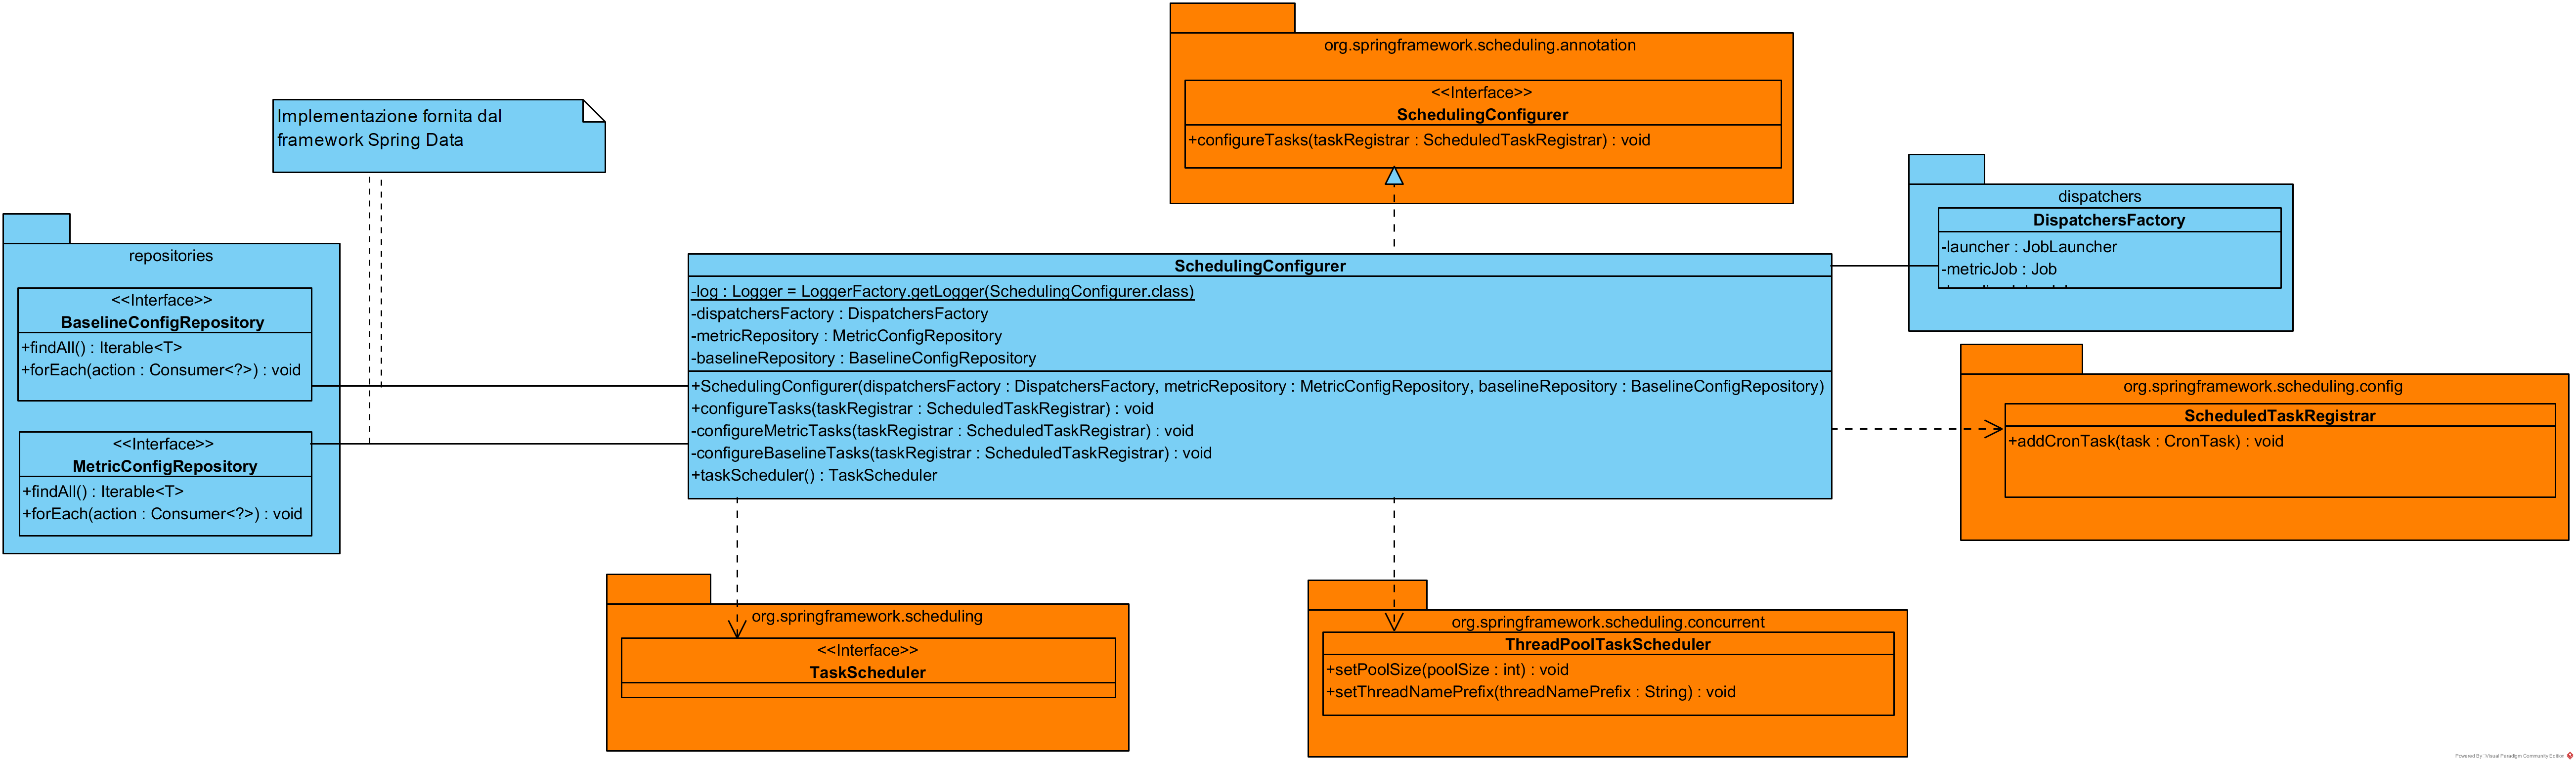
\includegraphics[width=\textwidth]{./img/DiagrammiClasse/SchedulingConfigurer.png}
   	        \caption[Diagramma della classe SchedulingConfigurer]{Diagramma della classe SchedulingConfigurer}
	    \end{figure}\\
        
        La classe SchedulingConfigurer si occupa di:
        \begin{itemize}
        	\item costruisce un oggetto \textit{DispatchersFactory} necessario per la costruzione di dispatchers;
        	\item costruisce un oggetto \textit{MetricConfigRepository} necessario per andare a prelevare da 
        		Elasticsearch la corretta configurazione per le metriche da creare;
        	\item costruisce un oggetto \textit{BaselineConfigRepository} necessario per andare a prelevare da 
        		Elasticsearch la corretta configurazione per le baseline da creare;
        	\item definire un oggetto \textit{TaskScheduler} necessario per la gestione dei task riguardanti
        		le metriche o le baseline all'interno dell'applicazione.
        \end{itemize}
        La classe implementa l'interfaccia \textit{SchedulerConfigurer} del framework Spring, documentata alla pagina
        \url{https://bit.ly/2IINkN8}. Questo perché permette di creare un oggetto \textit{TaskScheduler}
        capace di aggiungere operazioni alla coda delle operazioni da svolgere, la documentazione di questa 
        classe è presente all'indirizzo \url{https://bit.ly/2ksJbyi}. \\
        La classe utilizza le seguenti classi/interfacce:
        \begin{itemize}
        	\item \textbf{DispatchersFactory}: grazie a questa classe è possibile creare dispatchers che gestiscano la coda
        		dei processi;
        	\item \textbf{BaselineConfigRepositories}: permette di prelevare da Elasticsearch la configurazione prevista
        		per la costruzione di una baseline;
        	\item \textbf{MetricConfigRepositories}: permette di prelevare da Elasticsearch la configurazione prevista
        		per la costruzione di una metrica;
        	\item \textbf{TaskScheduler}: questa classe permette la programmazione di oggetti \textit{Runnables} in
        		base a diversi tipi di triggers;
        	\item \textbf{ThreadPoolTaskScheduler}: questa classe è l'implementazione dell'interfaccia \textit{TaskScheduler} 
				utilizzata in \ProjectName{};
        	\item \textbf{SchedulerTaskRegistrar}: è utilizzata come classe di supporto nella registrazione di 
        		operazioni nel \textit{TaskScheduler}.
        \end{itemize}
		
		
	
	    